% chapter1.tex {Introduction}

\chapter{Introduction}
\label{ch:intro}

This chapter provides an overall description of the field of work covered herein, as well as some outline for the remainder of the thesis.

The objective of this thesis is to introduce a new method --- or at least improve on existing methods --- for studying problems in network information flow. Linear coding methods have shown to be insufficient for certain solvable networks \cite{doug2005}, and many open questions still remain regarding linear coding as an approach \cite{riis2004, cann2006}. Open questions are indeed a feature of a number of recent publications in this relatively new field; however, each paper does go some way to reducing the overall number of these questions. This thesis aims to do the same.

The approach for this thesis will be to study the theories and technologies currently in use, and to investigate where and why they prove to be inadequate. By highlighting these points of failure it should be possible to work toward an optimal solution to overcome these problems. Before investigating the modern technologies in use, however, it is necessary to provide some introduction of the history of networking.

\section{Graph Theory}

Graph theory is an area of mathematics, often regarded as being popularised when Leonhard Euler solved the problem of the Seven Bridges of K{\"o}nigsberg \cite{bigg1986}. Euler's work, later generalised by other mathematicians, is said to be at the heart of topology, a branch of mathematics not introduced until over a century later. Graph theory contains a number of accessible problems, one of the most famous being the four colour theorem. This theorem is particularly famous due to the use of a computer to assist in the proof; the computer was used to show that only four colours were required for each of about $2000$ maps, to one of which any map could be reduced \cite{appe1977}. In fact, the four colour theorem (or its earlier forms and attempts to solve it) has been suggested as the origin of the entire field of graph theory \cite{wils2003}.

The use of a computer in proving mathematical theorems is a controversial issue, not least because of the lack of elegance in the proof. As with the four colour theorem, a computer is usually used to exhaustively prove a great number of cases that could not feasibly be produced by hand without years of computation. The objection to using computers in this manner is also that the proofs may not be logically verifiable, simply because of the number of steps. The algorithm and programs used must be fully trusted to accept the proof.

In addition to a number of colouring problems, there are various routing problems, some of which can be expressed as problems in computational complexity theory. Computational complexity theory is concerned with finding the most efficient algorithm to solve a given problem. An example is the travelling salesman problem, which seeks to find the Hamiltonian cycle with the least weight for a given complete weighted graph. In terms of computational complexity, finding such a cycle is \textbf{NP}-hard. A brute-force method for solving such a problem quickly becomes impractical, as the time required to find the shortest cycle grows with $n!$, where $n$ is the number of nodes in the graph. It is critical, then, to develop algorithms to solve these problems more efficiently. Investigations have demonstrated that both algorithms and network flow problems are closely related to the colouring problems mentioned above \cite{wils2003}.

\section{Information Theory}

Applied mathematics has long been used to solve problems in information theory. The discipline of information theory was formalised in~1948 by Claude Shannon \cite{shan1948}, though existing communication methods had used the ideas for some years previously. Information theory is based on probability theory and encompasses a number of scientific and engineering disciplines, and as such is a fundamental part of many modern developments and inventions, from mobile phones and compact discs to the study of black holes \cite{beke1973}. Network information theory is concerned with the study of networks --- or acyclic, directed graphs --- and the transmission of information in these networks.

At the heart of Shannon's work is coding theory, dealing with the transmission of information across a noisy channel. The codes are separated into two types; source coding and channel coding. Source coding seeks to compress the data so that fewer bits are required to transmit it. The fewest number of bits required to transmit a piece of information is given by its entropy (see Section~\ref{sect:entropy}). On the other hand, channel coding adds redundant data to minimise the effect of the noise. The redundant data are used as error correcting codes. The paper also states that reliable communication is possible (i.e., errors may be made arbitrarily small) over a noisy channel if the rate of communication is less than the capacity of the channel. This paper is concerned with both types of coding.

\section{Network Coding}

Recently a new field of information theory, known as \textbf{network coding}, has emerged. The concept was introduced by Ahlswede \textit{et al.}, and they give examples as to the benefits of using network coding to increase network throughput. The findings have significantly affected the discipline of information theory by showing that traditional routing methods do not suffice when attempting to achieve the optimal flow of a network \cite{ahls2000}. Work on this new area has advanced significantly over the past few years (see, for example, \cite{ahls2000, hoka2003, koet2003, riis2004, doug2005}).

Network coding has emerged as a result of the theories above --- initially developed for satellite communications \cite{yeun1999}, the tools introduced were new to multi-user information theory. Network theory uses graphs to represent relationships between discrete objects, and hence coincides with graph theory. Network coding builds on network routing, a problem in network theory, and shows that network routing is not sufficient (see Section~\ref{sect:netcod}).

\section{Origins of Work}

\begin{figure}[ht]
	\centering
	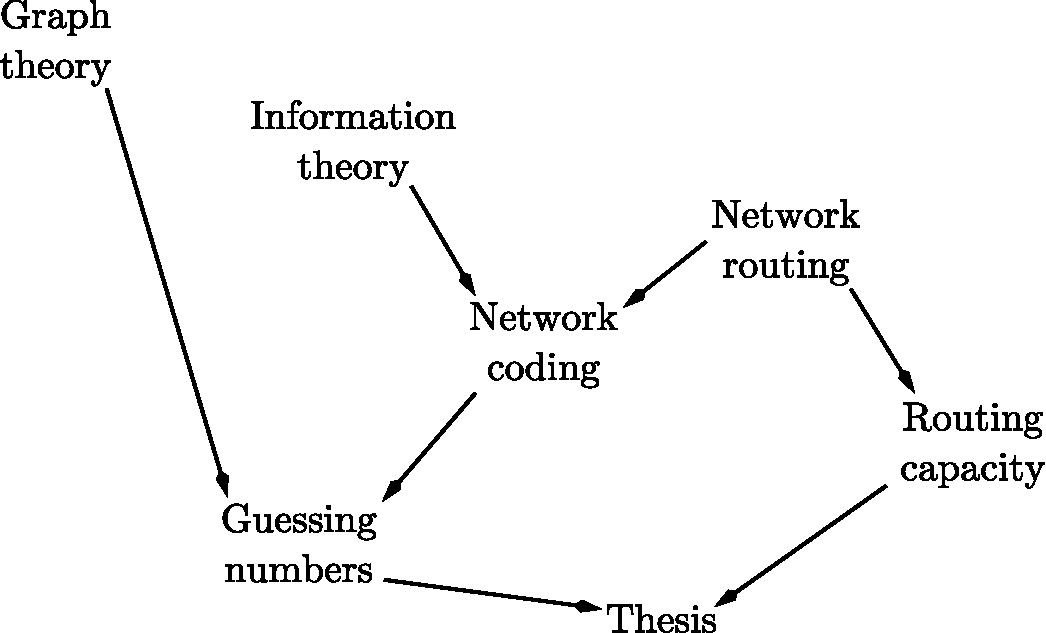
\includegraphics[width=.6\textwidth]{figures/history.pdf}
	\caption[History of the field and topic association]{Each topic builds upon another previous area of work. This diagram shows the association between topics covered, and how they lead to the work in this thesis.}
	\label{history}
\end{figure}

Figure~\ref{history} shows how the topics introduced above are relevant to the work in this thesis. Network coding builds on ideas from traditional network routing (Section~\ref{sect:routing}) and combines it with information theory. This thesis combines the new concept of \textbf{guessing numbers} \cite{riis2005util, riis2005info} (Section~\ref{sect:guessing_number}) and an existing subfield of network routing known as \textbf{routing capacity} (Section~\ref{sect:routing_capacity}). Each step can be seen as using the tools from one discipline to improve the techniques used in the other. For example, this thesis aims to use the tools used in routing capacity to improve on the concept of guessing numbers.

\section{Criteria for Success}
\label{sect:objective}

As mentioned at the beginning of this chapter, this thesis is concerned with producing a new or improved technique for dealing with information flow problems. Ideally, this technique should help to answer some of the open questions in the field of network coding. The criteria for success are outlined below and are evaluated in Chapter~\ref{ch:eval}.

\begin{itemize}
	\item{Study and description of existing methods within network coding and network routing capacity;}
 	\item{development of a new method for studying network flow problems based on existing techniques;}
 	\item{abstraction and formalisation of a modified guessing game based on the new method;}
 	\item{study and evaluation of cases in which the new game is more successful than the existing game.}
\end{itemize}

\section{Thesis Outline}

Chapter~\ref{ch:litrev} contains the literature review, defining some of the key concepts and discussing work in the fields of information theory and network coding. It describes how the shortcomings of traditional routing used in existing network technologies have brought about these new fields. In addition, it gives more detailed information on some of the open and solved problems. Specific attention is paid to three papers by Riis \textit{et al.} \cite{riis2005util, riis2005info, came2007}, the only previously submitted papers detailing the concept on which this thesis expands. The background study required to understand the methods used in later chapters is reviewed here.

Chapter~\ref{ch:prob} expands on some of the open problems mentioned in Chapter~\ref{ch:litrev}, together with other problems that were approached. As well as expanding and improving on existing work, it covers definitions of new concepts in the field. New definitions and propositions are provided here. In particular, the new concept of a ``routing guessing game'' allows certain problems in network information flow to be viewed with a new approach.

Chapter~\ref{ch:sol} provides examples and applications of these new ideas. In addition, the main theorems required to validate this new concept are proved here. Specifically, the existence of a non-integer guessing number is proved using a specific guessing strategy on the pentagon.

Chapter~\ref{ch:eval} provides a critical evaluation of the issues tackled and overcome throughout the writing of the thesis. It discusses whether the problems raised at the beginning of the thesis have been sufficiently addressed. The criteria for success are each evaluated in turn to provide a complete review of the work undertaken. The achievements of the thesis as well as its impact on the field of information theory are discussed in this chapter, as well as some possibilities for further work.

Chapter~\ref{ch:conc} provides conclusions from the ideas discussed in the thesis by giving a general review of the work undertaken. Open questions that have either arisen from the work contained herein or from previous work are listed in this final chapter.